\begin{name}
	{\tenchude}
	{TOÁN 10}
	{LỚP TOÁN THẦY PHÁT}
	{Thời gian: 90 phút - Không kể thời gian phát đề}
\end{name}
\TN
\Opensolutionfile{ans}[ans/ansDe1-TN1]
\begin{ex}%[0H9N3-1]
	Một đường thẳng có bao nhiêu vectơ pháp tuyến?
	\choice
	{$0$}
	{$1$}
	{$2$}
	{\True Vô số}
	\loigiai{
		Một đường thẳng có vô số vectơ pháp tuyến.
	}
\end{ex}

\begin{ex}%[0H9N3-3]
	Trong mặt phẳng tọa độ, cho hai đường thẳng có phương trình
	$\Delta_1 \colon x - y + 1 = 0$, $\Delta_2 \colon 2x - 2y + 3 = 0$. Khi đó
	\choice
	{ $\Delta_1 \equiv \Delta_2$}
	{ $\Delta_1 \perp \Delta_2$}
	{ $\Delta_1$ cắt và không vuông góc với $\Delta_2$}
	{\True $\Delta_1 \parallel \Delta_2$}
	\loigiai{
		Ta có $\dfrac{1}{2} = \dfrac{-1}{-2} \ne \dfrac{1}{3}$. Suy ra $\Delta_1 \parallel \Delta_2$.
	}
\end{ex}

\begin{ex}%[0H9N4-1]
	Điểm nào sau đây thuộc đường tròn $(O)\colon 2x^2+2y^2-4x-6y=6$?
	\choice
	{$(4,1)$}
	{$(3,2)$}
	{$(2,3)$}
	{\True $(1;4)$}
	\loigiai{Ta có
		$(1;4)$ thuộc $(O)$ vì $2\cdot 1^2+2\cdot 4^2-4\cdot 1-6\cdot 4=6$.}
\end{ex}

\begin{ex}%[0H9N4-1]
	Trong các phương trình sau, phương trình nào là phương trình của một đường tròn?
	\choice
	{$x^2+y^2+2x-4y+9=0$}
	{$x^2+y^2-6x+4y+13=0$}
	{\True $2x^2+2y^2-8x-4y-6=0$}
	{$5x^2+4y^2+x-4y+1=0$}
	\loigiai{
		\begin{itemize}
			\item Xét phương trình $x^2+y^2+2x-4y+9=0$ có $(-1)^2+2^2=5<9$ nên phương trình đã cho không là phương trình đường tròn.
			\item Xét phương trình $x^2+y^2-6x+4y+13=0$ có $3^2+2^2=13$ nên phương trình đã cho không là phương trình đường tròn.
			\item Xét phương trình $2x^2+2y^2-8x-4y-6=0 \Leftrightarrow x^2+y^2-4x-2y-3=0$ có $2^2+1^2=5>-3$ nên phương trình đã cho là phương trình đường tròn.
			\item Phương trình $5x^2+4y^2+x-4y+1=0$ không có dạng $x^2+y^2-2ax-2by+c=0$ nên không phải là phương trình đường tròn.
		\end{itemize}
	}
\end{ex}

\begin{ex}%[0H9N4-1]
	Trong mặt phẳng $O x y$, tọa độ tâm $I$ và bán kính $R$ của đường tròn
	$(C)\colon (x+1)^2+y^2=8$ là
	\choice[2]
	{$I(-1 ; 0)$, $R=8$}
	{$I(-1 ; 0)$, $R=64$}
	{\True $I(-1 ; 0)$, $R=2 \sqrt{2}$}
	{$I(1; 0)$, $R=2 \sqrt{2}$}
	\loigiai{Đường tròn
		$(C)\colon (x+1)^2+y^2=8$ có tọa độ tâm $I(-1;0)$ và bán kính $R=2\sqrt{2}$.}
\end{ex}

\begin{ex}%[0H9N5-2]%[Dự án đề kiểm tra Toán 10 HKII NH23-24-TrungKien]%[THPT TranHungDao-TPHCM]
	Phương trình nào sau đây là phương trình chính tắc của đường elip?
	\choice
	{$\dfrac{x^2}{2}+\dfrac{y^2}{5}=1$}
	{$\dfrac{x^2}{8}+\dfrac{y^2}{8}=1$}
	{\True $\dfrac{x^2}{4}+\dfrac{y^2}{1}=1$}
	{$\dfrac{x^2}{3}-\dfrac{y^2}{1}=1$}
	\loigiai{
		Phương trình $\dfrac{x^2}{4}+\dfrac{y^2}{1}=1$ có $a=2>b=1>0$ là một phương trình chính tắc của elip.
	}
\end{ex}

\begin{ex}%[0H9N5-5]
	Phương trình nào sau đây là phương trình của đường hypebol?
	\choice
	{\True $\dfrac{x^2}{9} - \dfrac{y^2}{16} = 1$}
	{$\dfrac{x^2}{9} + \dfrac{y^2}{16} = 1$}
	{$\dfrac{x^2}{9} - \dfrac{y^2}{16} = 0$}
	{$\dfrac{x^2}{9} + \dfrac{y^2}{16} = 0$}
	\loigiai{
		$\dfrac{x^2}{9} - \dfrac{y^2}{16} = 1$ là dạng đúng phương trình của một hypebol.
	}
\end{ex}

\begin{ex}%[0H9N5-7]
	Parabol $y^2=\dfrac{3}{2}x$ có đường chuẩn là
	\choice
	{$x=-\dfrac{3}{4}$}
	{$x=\dfrac{3}{4}$}
	{$x=\dfrac{3}{2}$}
	{\True $x=-\dfrac{3}{8}$}
	\loigiai{
		Phương trình chính tắc của parabol $(P)\colon y^2=2px$
		$\Rightarrow p=\dfrac{3}{4}$.\\
		Vậy phương trình đường chuẩn là $x=-\dfrac{p}{2}=-\dfrac{3}{8}$.
	}
\end{ex}

\begin{ex}%[Mức 2]%[0D3N1-4]
	Đồ thị hàm số $y=\sqrt{3-2x}$ đi qua điểm nào trong các điểm sau đây?
	\choice
	{\True $C(-3;3)$}
	{$A(3;3)$}
	{$B(-2;1)$}
	{$D(2;-1)$}
	\loigiai
	{Ta có $y(-3)=\sqrt{3-2\cdot (-3)}=\sqrt{9}=3$ nên đồ thị hàm số đi qua điểm $C(-3;3)$.}
\end{ex}

\begin{ex}%[0D3N1-5]
	Trong các hàm số sau, hàm số nào đồng biến trên khoảng $(-2;0)$?
	\choice
	{\True $y=x$}
	{$y=\dfrac{1}{x}$}
	{$y=|x|$}
	{$y=x^2$}
	\loigiai{Ta có hàm số $y=x$ là hàm số đồng biến trên $\mathbb{R}$ nên hàm số $y=x$ tăng trên $(-2;0)$.}
\end{ex}

\begin{ex}%[Đề thi HK1 trường Song Ngữ Á Châu năm học 2023-2024]%[Trần Quang Trường, dự án 10-11EX]%[0D3N2-1]
	Cho hàm số bậc hai $y=ax^2+bx+c$ $(a\ne 0)$ có đồ thị $(P)$, đỉnh của $(P)$ được xác định bởi công thức nào?
	\choice
	{\True $I\left(-\dfrac{b}{2a}; -\dfrac{\Delta}{4a}\right)$}
	{$I\left(-\dfrac{b}{a}; -\dfrac{\Delta}{4a}\right)$}
	{$I\left(\dfrac{b}{2a}; \dfrac{\Delta}{4a}\right)$}
	{$I\left(-\dfrac{b}{2a}; \dfrac{\Delta}{4a}\right)$}
	\loigiai{

	}
\end{ex}

\begin{ex}%[Dự án EX-10-11-Chuẩn hóa]%[Hoàng Thanh Phương]%[0D3N2-2]
	Cho hàm số $y=x^2-4x+7$. Trong những mệnh đề sau đây mệnh đề nào là mệnh đề đúng?
	\choice{\True Hàm số đồng biến trên khoảng $(3;+\infty)$}{Hàm số đồng biến trên $(-\infty;2)$}{Hàm số đồng biến trên khoảng $(-\infty;-2)$}{Hàm số nghịch biến trên $\mathbb{R}$}
	\loigiai{
		Bảng biến thiên của hàm số $y=x^2-4x+7$ như sau
		\begin{center}
			
\begin{tikzpicture}
				\tkzTabInit[lgt=1.2,espcl=3]
				{$x$/0.8,$y$/2.3}
				{$-\infty$,$2$,$+\infty$}
				\tkzTabVar{+/$+\infty$,-/$3$,+/$+\infty$}
			\end{tikzpicture}
		\end{center}
		Dựa vào bảng biến thiên, hàm số đồng biến trên khoảng $(2;+\infty)$ nên đồng biến trên khoảng $(3;+\infty)$.
	}
\end{ex}
\Closesolutionfile{ans}

\TNTF
\Opensolutionfile{ans}[ans/ansDe1-TN2]
\begin{ex}%[0H9H3-2]%[0H9H3-3]
	Trong mặt phẳng tọa độ $Oxy$, cho đường thẳng $d_1\colon x-2y+3=0$, $d_2\colon 3x-y-1=0$ và điểm $A(2;1)$.
	\choiceTF
	{Đường thẳng $d_1$ đi qua điểm $A$}
	{\True Đường thẳng $d_1$ có một vectơ chỉ phương là $\overrightarrow{u}_1=(2;1)$}
	{\True Hai đường thẳng $d_1$ và $d_2$ cắt nhau tại điểm $M(1;2)$}
	{Góc giữa hai đường thẳng $d_1$ và $d_2$ là $\dfrac{\sqrt 2}{2}$}
	\loigiai{
		\begin{itemchoice}
			\itemch {\bf Sai}.\\
			Vì $2-2\cdot 1+3 \ne 0$ nên đường thẳng $d_1$ không đi qua điểm $A$.
			\itemch {\bf Đúng}.\\
			Vì $d_1\colon x-2y+3=0$ nên $d_1$ có một vectơ pháp tuyến là $\overrightarrow{n}_1=(1;-2)$. Nên $d_1$ có một vectơ chỉ phương là $\overrightarrow{u}_1=(2;1) \perp \overrightarrow{n}_1$.
			\itemch {\bf Đúng}.\\
			Giao điểm của $d_1$ và $d_2$ là nghiệm của hệ phương trình $\heva{&x-2y+3=0\\&3x-y-1=0.}$\\
			Giải hệ ta được $\heva{&x=1\\&y=2.}$\\
			Vậy, hai đường thẳng $d_1$ và $d_2$ cắt nhau tại điểm $M(1;2)$.
			\itemch {\bf Sai}.\\
			Ta có một vectơ pháp tuyến của $d_1$ là $\overrightarrow{n}_1=(1;-2)$; một vectơ pháp tuyến của $d_2$ là $\overrightarrow{n}_2=(3;-1)$.\\
			Khi đó, $\cos (d_1,d_2)=\dfrac{|\overrightarrow{n}_1\cdot \overrightarrow{n}_2|}{|\overrightarrow{n}_1|\cdot |\overrightarrow{n}_2|}=\dfrac{|1\cdot 3+(-2)\cdot (-1)|}{\sqrt{1^2+(-2)^2}\cdot \sqrt{3^2+(-1)^2}}=\dfrac{5}{5\sqrt 2}=\dfrac{\sqrt 2}{2}$.\\
			Suy ra, $(d_1,d_2)=45^\circ$.
		\end{itemchoice}
	}
\end{ex}

\begin{ex}%[0-HK1-CD-1-SoBacNinh-2324]%[VN-MT-6, Tống Văn Ký]%[0D3H1-2]
	Cho hàm số $f(x)=3-2x$ và hàm số $g(x)=x^2-x+1$.
	\choiceTF
	{Hàm số $f(x)$ đồng biến trên khoảng $(-\infty; \dfrac{3}{2})$}
	{\True Đồ thị hàm số $f(x)$ đi qua điểm $A(1;1)$}
	{Đồ thị hàm số $g(x)$ cắt trục $Ox$ tại hai điểm phân biệt}
	{Đồ thị hàm số $g(x)$ cắt đồ thị hàm số $f(x)$ tại hai điểm phân biệt có tổng tung độ bằng $0$}
	\loigiai{
		\begin{itemchoice}
			\itemch {\bf Sai.}\\
			Vì $a=-2<0$ nên hàm số $f(x)$ nghịch biến trên $\mathbb{R}$.
			\itemch {\bf Đúng.}\\
			Vì $f(1)=3-2\cdot 1=1$ nên đồ thị hàm số $f(x)$ đi qua điểm $A(1;1)$.
			\itemch {\bf Sai.}\\
			Vì $\Delta=1^2-4\cdot 1\cdot 1=-3<0$ nên phương trình $g(x)=0$ vô nghiệm hay đồ thị hàm số $g(x)$ không cắt trục $Ox$.
			\itemch {\bf Đúng.}\\
			Ta có $f(x)=g(x) \Leftrightarrow 3-2x=x^2-x+1 \Leftrightarrow x^2+x-2=0 \Leftrightarrow x=-2$ hoặc $x=1$.\\
			Vậy, đồ thị hàm số $g(x)$ cắt đồ thị hàm số $f(x)$ tại hai điểm phân biệt có tung độ lần lượt là $f(1)=1$ và $f(-2)=7$. Nên tổng tung độ của hai điểm đó bằng $8$.
		\end{itemchoice}
	}
\end{ex}
\Closesolutionfile{ans}

\TNSA
\Opensolutionfile{ans}[ans/ansDe1-TN3]
\begin{ex}%[0H9H3-2]
	Cho đường thẳng $d$ có phương trình tham số là $\heva{&x=1+3t\\&y=2-t}$. Biết phương trình tổng quát của $d$ là $ax+by+11=0$. Tính $a+b$.
	\shortans{$-4$}
	\loigiai{
		Ta có $d\colon \heva{&x=1+3t\\&y=2-t}$. Suy ra $d$ đi qua điểm $A(1;2)$ và có vectơ chỉ phương $\overrightarrow{u}=(3;-1)$ nên $d$ có vectơ pháp tuyến $\overrightarrow{n}=(1;3)$.\\
		Phương trình tổng quát của $d$ là $1 \cdot (x-1)+3\cdot (y-2)=0 \Leftrightarrow x+3y-7=0 \Leftrightarrow -\dfrac{11}{7}x-\dfrac{33}{7}y+11=0$.\\
		Vậy $a+b=-\dfrac{44}{7} \approx -6,3$.
	}
\end{ex}

\begin{ex}%[0H9V4-2]
	Cho đường tròn $(C)$ có tâm $I(1;2)$ và một tiếp tuyến $d \colon 3x+y+5=0$. Tính chu vi đường tròn $C$ (kết quả làm tròn đến hàng phần chục).
	\shortans{$19{,}9$}
	\loigiai{
		Ta có $I(1;2)$ là tâm của đường tròn $(C)$ và $d \colon 3x+y+5=0$ là tiếp tuyến của đường tròn $(C)$ nên $(C)$ có bán kính bằng
		$$R=\mathrm{d}(I,d)=\dfrac{|3\cdot 1 + 2 +5|}{\sqrt{3^2+1^2}}=\dfrac{10}{\sqrt{10}}=\sqrt{10}.$$
		Vậy chu vi của đường tròn $(C)$ là $2\pi R=2\pi \sqrt{10}\approx 19{,}9$.
	}
\end{ex}

\begin{ex}%[0H9V3-8]
	\immini
	{
	Một ao cá có dạng hình chữ nhật $ABCD$ với chiều dài $AD=17$\,m, chiều rộng $AB=13\,$m. Phần tam giác $DEF$ người ta để nuôi vịt, biết $AE=6\,$m, $CF=6{,}5\,$m (minh họa như hình vẽ). Tính khoảng cách từ vị trí người đứng câu cá ở vị trí $B$ đến vách ngăn nuôi vịt là đường thẳng $EF$. (Kết quả làm tròn đến hàng phần chục).
	}
	{\begin{tikzpicture}[scale=0.4, font=\footnotesize, line join = round, line cap = round,>=stealth]
		\path
		(-4,0) coordinate (B)
		(-4,7) coordinate (A)
		(3,0) coordinate (C)
		(3,7) coordinate (D)
		(-5/3,7) coordinate (E)
		(3,3.5) coordinate (F);
		\draw[fill=black!30!green,opacity=0.6]
		(-5,-1.5)
		.. controls ++(90:0.1) and ++(180: 1) .. (-5,8)
		.. controls ++(180:0.1) and ++(90: 1) .. (5.5,8)
		.. controls ++(90:0.1) and ++(100: 1) .. (5.5,-1.5)
		.. controls ++(180:0.1) and ++(30: 1) .. (-5,-1.5);
		\draw[fill=green!50] plot[smooth cycle] coordinates{(5.11,1.14)(5.87,1.01) (6.09,1.88) (5.93,2.62) (6.03,3.31)(5.5,3.65)(5.37,4.45)(5,5)(4.66,4.29)(4.29,3.55)(4.5,2.88)(3.94,2.62)(3.81,1.8)(4.23,1.24)(4.82,1.19)};
		\draw[fill=black!70] plot[smooth ] coordinates{(5.3,0)(5.25,1.14)(5.25,1.8)(5.7,2.9)(5.18,2.05)(5.09,4.2)(5.06,2.3)(5.0,1.65)(4.2,2.4)(5.01,1.29) (5,0) };
		\fill[cyan!30]  (-4,0) rectangle (3,7);
		\draw (A)--(B)--(C)--(D)--cycle;
		\draw[red]  (E)--(F);
		\node[scale=2.3,yscale=2] at (-4.2,1){\faBlind};
		\draw (-3.5,-0.4)
		.. controls ++(30:0.1) and ++(70: 1) .. (-2,1);
		\foreach \y in {0,60,...,720} {
				\draw[color=white] (0.5,6.5)--++(\y:.1) (1.5,6.5)--++(\y:.1) (2.5,6.5)--++(\y:.1)
				(1,5.7)--++(\y:.1) (2,5.7)--++(\y:.1) (2.7,5.7)--++(\y:.1)
				(1.8,4.7)--++(\y:.1)(2.6,4.7)--++(\y:.1);}
		\foreach \p/\r in {B/-90,C/-90,F/0,D/60,E/90,A/110}
		\fill[color=white] (\p) circle (1.5pt) node[shift={(\r:3mm)}]{$\p$};
		\draw[->] (-6,0)--(7,0)node[above]{$x$};
		\draw[->] (-4,-2)--(-4,10)node[left]{$y$};
	\end{tikzpicture}
	}
	\shortans[]{$14{,}2$}
	\loigiai{
	Chọn hệ trục tọa độ $Oxy$ có $O$ trùng với $B$, các tia $Ox$, $Oy$ tương ứng trùng với các cạnh $BC,BA$. Chọn một đơn vị độ dài trên mặt phẳng tọa độ ứng với $1\,$m trong thực tế.\\
	Khi đó $A(0;13), B(0;0),C(17;0), D(17;13), E(6;13), F(17;6{,}5)$.\\
	$\vec{EF}=(11;-6{,}5)\Rightarrow \vec{n}=(6{,}5;11) $.\\
	Phương trình	$EF\colon 6{,}5(x-6)+11(y-13)=0\Leftrightarrow EF\colon 6{,}5x+11y-182=0$.\\
	Khoảng cách từ $B$ đến $(EF)$ là $\mathrm{d}(B,EF)=\dfrac{|-182|}{\sqrt{6{,}5^2+11^2}}\approx 14{,}2$.\\
	Vậy khoảng cách từ vị trí người đứng câu cá đến vách ngăn nuôi vịt là $14{,}2\, $m.
	}

\end{ex}

\begin{ex}%[0H9V5-0]
	\immini
	{
		Một chiếc đèn có mặt cắt ngang là hình parabol $y^2=2px\ (p>0)$ như hình vẽ. Trong đó chiều rộng hai mép vành là $AB=40$ cm, chiều sâu $h=20$ cm (khoảng cách từ $O$ đến $AB$), bóng đèn nằm ở tiêu điểm $S$. Tính khoảng cách từ bóng đèn đến đỉnh $O$ của vành đèn.
		\shortans{$5$}
	}
	{
		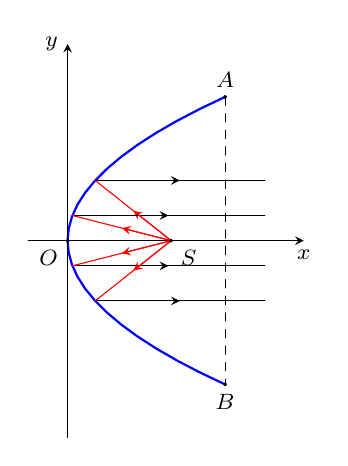
\begin{tikzpicture}[scale=0.5, font=\footnotesize, line join=round, line cap=round, >=stealth]

			\draw[domain=-3.65:3.65, blue,thick] plot({3/10*(\x)^2},\x);
			%\draw[gray!10] (-1,-1) grid (5,5);
			\draw[->] (-1,0)--(6,0) node[below]{$x$};
			\draw[->] (0,-5)--(0,5) node[left]{$y$};
			\coordinate (A) at (4,3.65);
			\coordinate (B) at (4,-3.65);
			\coordinate (O) at (0,0);
			\coordinate (C) at (0.12,0.64);
			\coordinate (C') at (0.12,-0.64);
			\coordinate (D) at (0.7,1.53);
			\coordinate (D') at (0.7,-1.53);
			\coordinate (F) at (5.01,1.53);
			\coordinate (F') at (5.01,-1.53);
			\coordinate (G) at (5.01,0.64);
			\coordinate (G') at (5.01,-0.64);
			\coordinate (E) at (2.63,0);
			\coordinate (H1) at (1.67,0.76);
			\coordinate (H2) at (1.67,-0.76);
			\coordinate (H3) at (1.38,0.32);
			\coordinate (H4) at (1.38,-0.32);
			\coordinate (K1) at (2.85,1.53);
			\coordinate (K2) at (2.85,-1.53);
			\coordinate (K3) at (2.56,0.64);
			\coordinate (K4) at (2.56,-0.64);
			\draw  (F)--(D) (G)--(C) (F')--(D') (G')--(C') ;
			\draw[dashed] (A)--(B);
			\draw[red,->] (E)--(H1);
			\draw[->] (D)--(K1) ;
			\draw[red,->] (E)--(H3);
			\draw[->] (C)--(K3) ;
			\draw[red,->] (E)--(H4);
			\draw[->] (C')--(K4) ;
			\draw[red,->] (E)--(H2);
			\draw[->] (D')--(K2) ;

			\draw[red] (E)--(C) (E)--(D) (E)--(C') (E)--(D');

			\draw[fill=black] (A) circle (1pt) node [above] {$A$};
			\draw[fill=black] (B) circle (1pt) node [below] {$B$};
			\draw[fill=black] (E) circle (1pt) node [below right] {$S$};
			\draw[fill=black] (O) circle (1pt) node [below left] {$O$};
		\end{tikzpicture}
	}
	\loigiai{
		Từ giả thiết ta có parabol đi qua điểm $A(20;20)$ thay vào phương trình $y^2=2px$ do đó $20^2=2p\cdot 20\Leftrightarrow  p=10$.\\
		Nên $OS=\dfrac{p}{2}=5$.}
\end{ex}
\Closesolutionfile{ans}

\TL
\begin{ex}%[THPT Lê Thánh Tông - TP HCM, 2023-2024]%[Toàn Phan, 10-11EXHK1]%[0D3H2-3]
	Vẽ đồ thị hàm số $y=2x^2-4x+3$.
	\loigiai{
		Ta có $a=2$, $b=-4$, $c=3$ $\Rightarrow -\dfrac{b}{2a}=1$ và $-\dfrac{\Delta}{4a}=1$.\\
		Đồ thị hàm số $y=2x^2-4x+3$ là một parabol có
		\begin{itemize}
			\item Đỉnh $I\left(1;1\right)$,
			\item Trục đối xứng $x=1$,
			\item Bề lõm hướng lên (vì $a>0$),
			\item Bảng giá trị:
			      \begin{center}
				      \begin{tabular}{|c|c|c|c|c|c|c|c|c|c|c|}
					      \hline
					      $x$ & $-1$ & $0$ & $1$ & $2$ & $3$ \\
					      \hline
					      $y$ & $9$  & $3$ & $1$ & $3$ & $9$ \\
					      \hline
				      \end{tabular}
			      \end{center}
		\end{itemize}
		Đồ thị
		\begin{center}
			\begin{tikzpicture}[scale=1, font=\footnotesize, line join=round, line cap=round,>=stealth]
				\draw[->] (-2,0)--(4,0) node[below]{$x$};
				\draw[->] (0,-1)--(0,10) node[left]{$y$};
				\draw[domain=-1.05:3.05,smooth,variable=\x, thick] plot (\x,{2*(\x)^2-4*\x+3});
				\foreach \i in {-1,1,2,3}
				\draw (\i,0) node[below]{$\i$};
				\foreach \i in {-1,1,2,...,9}
				\draw (0,\i) node[left]{$\i$};
				\draw[dashed] (1,-.5)node[right]{$x=1$}--(1,9.5);
			\end{tikzpicture}
		\end{center}
	}
\end{ex}

\begin{ex}%[0H9V3-8]%[Dự án đề 4 phần]$%[Tex hóa: Lê Thị Thúy Hằng]
	\immini[thm]{Nhà bạn Nam muốn đổi tủ lạnh và dự định kê vào vị trí dưới cầu thang. Biết vị trí định kê tủ lạnh có mặt cắt là một hình thang vuông với hai đáy lần lượt là $250$ cm và $150$ cm, chiều cao là $150$ cm (như hình vẽ). Bố mẹ Nam định mua một chiếc tủ lạnh có chiều cao $183$ cm và bề ngang $90$ cm. Bằng cách sử dụng phương pháp tọa độ, hãy tính xem nếu bố mẹ Nam kê chiếc tủ lạnh mới cách vách trái $2$ cm thì mép trên của tủ lạnh còn cách cầu thang theo phương thẳng đứng tối thiểu bao nhiêu cm? (tham khảo hình vẽ).
	}{
		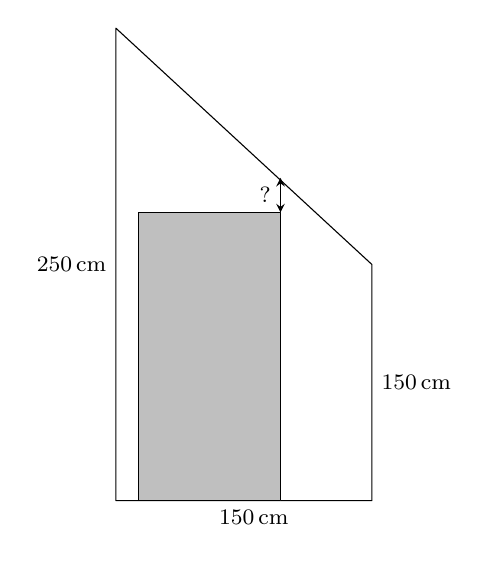
\begin{tikzpicture}[scale=1, font=\footnotesize, line join=round, line cap=round,>=stealth]
			\draw (-0.25,0)--(3,0)--(3,3)--(-0.25,6)--cycle;
			\draw[fill=gray!50](0.04,0) rectangle (1.84,3.66);
			\draw[<->] (1.84,3.66)--(1.84,4.1) node[midway, left]{$?$};
			\path
			(0,0)--(3,0) node[midway, below]{$150$\,cm}
			(3,0)--(3,3) node[midway, right]{$150$\,cm}
			(-0.25,0)--(-0.25,6) node[midway, left]{$250$\,cm}
			;
		\end{tikzpicture}
	}
	\loigiai{
		Gọi $A$, $B$, $C$, $M$, $N$ là các điểm có vị trí và tọa độ như trên hình.
		\begin{center}
			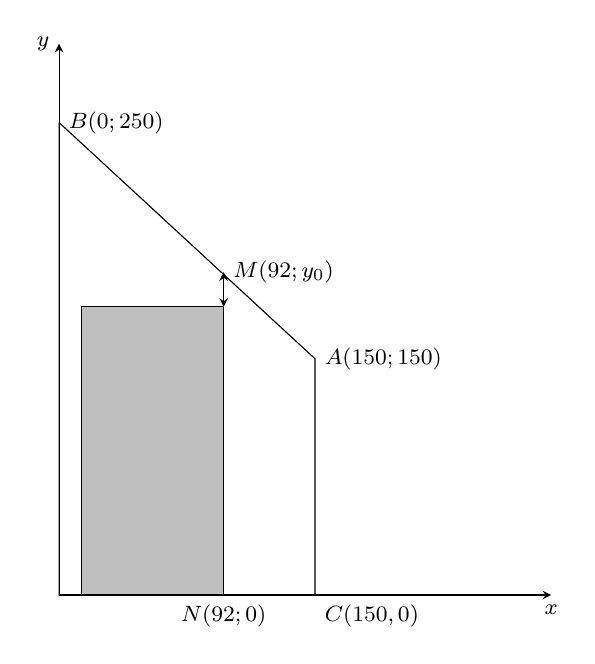
\begin{tikzpicture}[scale=1, font=\footnotesize, line join=round, line cap=round,>=stealth]
				\draw[->] (-0.25,0)--(6,0) node[below]{$x$};
				\draw[->] (-0.25,0)--(-0.25,7) node[left]{$y$};
				\draw (-0.25,0)--(3,0)--(3,3)--(-0.25,6)--cycle;
				\draw[fill=gray!50](0.04,0) rectangle (1.84,3.66);
				\draw[<->] (1.84,3.66)--(1.84,4.1);
				\path (-0.25,6)node[right]{$B(0;250)$}
				(1.84,4.1)node[right]{$M(92;y_0)$}
				(3,3)node[right]{$A(150;150)$}
				(3,0)node[below right]{$C(150,0)$}
				(1.84,0)node[below]{$N(92;0)$}
				;
			\end{tikzpicture}
		\end{center}
		Phương trình đường thẳng $AB$ là $2x+3y-750=0$.\\
		Điểm $M(92;y_M)$ thuộc đường thẳng $AB$ nên ta có \[2\cdot 92+3\cdot y_M-750=0\Rightarrow y_M=\dfrac{566}{3}.\]
		Vậy mép trên của tủ lạnh còn cách cầu thang theo phương thẳng đứng tối thiểu khoảng $\dfrac{566}{3}-183=\dfrac{17}{3}$ (cm).
	}
\end{ex}

\begin{ex}%[0D3C2-6]
	Một doanh nghiệp tư nhân $A$ chuyên kinh doanh xe gắn máy các loại. Hiện nay doanh nghiệp đang tập trung chiến lược vào kinh doanh xe hon đa Future Fi với chi phí mua vào một chiếc là $27$ triệu đồng và bán ra với giá là $31$ triệu đồng. Với giá bán này thì số lượng xe mà khách hàng sẽ mua trong một năm là $600$ chiếc. Nhằm mục tiêu đẩy mạnh hơn nữa lượng tiêu thụ dòng xe đang ăn khách này, doanh nghiệp dự định giảm giá bán và ước tính rằng nếu giảm $1$ triệu đồng mỗi chiếc xe thì số lượng xe bán ra trong một năm là sẽ tăng thêm $200$ chiếc. Vậy doanh nghiệp phải định giá bán mới là bao nhiêu để sau khi đã thực hiện giảm giá, lợi nhuận thu được sẽ là cao nhất. 
	% \shortans{$30{,}5$}
	\loigiai{
		Gọi $x$ đồng là số tiền mà doanh nghiệp A dự định giảm giá; $(0\le x\le 4)$.\\
		Khi đó\\
		Lợi nhuận thu được khi bán một chiếc xe là $31-x-27=4-x$.\\
		Số xe mà doanh nghiệp sẽ bán được trong một năm là $600+200x$.\\
		Lợi nhuận mà doanh nghiệp thu dược trong một năm là
		$$f(x)=(4-x)(600+200x)=-200x^2+200x+2400.$$
		Xét hàm số $f(x)=-200x^2+200x+2400$ trên đoạn $[0;4]$.\\
		TXĐ $\mathscr{D}=\mathbb{R}$.\\
		Đỉnh $I\left(\dfrac{1}{2};2450\right)$.\\
		Ta có bảng biến thiên:
		\begin{center}
			
\begin{tikzpicture}
				\tkzTabInit[lgt=3]
				{ $x$/1 , $f(x)$/2.5 }
				{ $-\infty$, $\dfrac{1}{2}$, $+\infty$}
				\tkzTabVar{ -/$-\infty$ , +/$2450$, -/$-\infty$}
				\tkzTabVal {1}{2}{0.5}{$0$}{$2400$}
				\tkzTabVal {2}{3}{0.5}{$4$}{$0$}
			\end{tikzpicture}
		\end{center}
		Vậy $\max\limits_{[0.4]} f(x)=2450\Leftrightarrow x=\dfrac{1}{2}$.
		Tức là khi giảm giá mỗi xe đi $0{,}5$ triệu đồng thì số xe bán ra được nhiều nhất.\\
		Vậy giá mới của chiếc xe là $30{,}5$ triệu đồng thì lợi nhuận thu được là cao nhất.
	}
\end{ex}

% \HetDe
% \label{De1}
% %
% \cleardoublepage
% \setcounter{page}{1}
% \rfoot{Trang \thepage/\pageref{DA1} - Đáp án trắc nghiệm Mã đề 1}
% \begin{center}
% 	\bfseries ĐÁP ÁN TRẮC NGHIỆM MÃ ĐỀ 1
% \end{center}

% \inputansbox{10}{ans/ansDe1-TN1}
% \inputansbox[3]{2}{ans/ansDe1-TN2}
% \inputansbox{3}{ans/ansDe1-TN3}
% \label{DA1}
% %
